% 0374(본책 70쪽) — 지름 AB 인 원 O 에 내접하는 □ABCD(색칠), DA∥CO, DA=6 cm. 답(넓이)은 적지 않는다. 스캔 삽화를 TikZ 로 다시 그림.
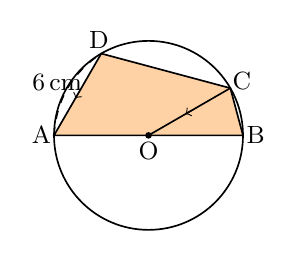
\begin{tikzpicture}[line width=0.6pt]
  \fill[orange!35] (-1.200,0.000) -- (1.200,0.000) -- (1.039,0.600) -- (-0.600,1.039) -- cycle;
  \draw (0.000,0.000) circle (1.200);
  \draw (-1.200,0.000) -- (1.200,0.000) -- (1.039,0.600) -- (-0.600,1.039) -- cycle;
  \draw (1.039,0.600) -- (0.000,0.000);
  \fill (0.000,0.000) circle (1.2pt);
  \draw[line width=0.4pt, ->] (-0.870,0.572) -- (-0.930,0.468);
  \draw[line width=0.4pt, ->] (0.572,0.330) -- (0.468,0.270);
  \draw[dashed, line width=0.4pt] (-1.200,0.000) to[bend left=25] (-0.600,1.039);
  \node[font=\small, inner sep=1.5pt] at (-1.160,0.670) {$6\,\mathrm{cm}$};
  \node[font=\small, inner sep=1.5pt] at (-1.360,0.000) {A};
  \node[font=\small, inner sep=1.5pt] at (1.360,0.000) {B};
  \node[font=\small, inner sep=1.5pt] at (1.186,0.685) {C};
  \node[font=\small, inner sep=1.5pt] at (-0.630,1.207) {D};
  \node[font=\small, inner sep=1.5pt] at (0.000,-0.200) {O};
\end{tikzpicture}
